\section{Importing Data from S3 to DynamoDB - Zhi Jiang}
This portion describes how I import data from data storage into a database for this project. Specifically, I need to read the file containing data in S3 and then import this data into a specified table in DynamoDB. In this document, I would like to talk about how to implement this portion, what problems I encountered and how to solve them.

\subsection{Create Table}
When implementing this function, EC2, as a server, is used to connect S3 and DynamoDB. In other words, we can execute scripts or programs on EC2 to access data in these services and operate these data among them. In fact, there are many kinds of method to implement our functions on the server such as Python, Java or other frameworks. We chose Python because we were familiar with this kind of language. On the other hand, Amazon Web Services provide a library Boto3, which has many useful methods to deal with these services such as creating a table or accessing data.\\

\noindent The first step is to create a table. boto3 has provided useful methods to complete this portion. In following codes, this is a standard template to create a table. First of all, we access our dynamoDB and then create a table object. We set the table name and some properties of an attribute such as name and type. We still set capacity for this table.\\ 
\begin{lstlisting}[language=Python, caption=create table]
dynamodb = boto3.client('dynamodb')

# create table 
table = dynamodb.create_table(
    # set name of table
    TableName = tname,
    # set information about attribute
    KeySchema = [
        {
            'AttributeName': 'PIN',
            'KeyType': 'HASH'
        }
    ],
    AttributeDefinitions = [
        {
            'AttributeName': 'PIN',
            'AttributeType': 'S'
        }
    ],
    ProvisionedThroughput = {
        'ReadCapacityUnits': 5,
        'WriteCapacityUnits': 5
    }
)
\end{lstlisting}

\subsection{Read Data}
\noindent The second step is we should read data of the original file from S3, but we used an incorrect method to read data at the beginning. The following codes are an improper way to access data in S3. We were not familiar with this SDK, so we through each file should be regarded as an object, and then we just need to read the content of this object. But eventually, we failed to read data from variable “content.”  In fact, we did not completely understand the role of an object type in this SDK. Object type is a complex constructor, and it contains much information.\\
\begin{lstlisting}[language=Python, caption=inappropriate method to access S3 and read data]
	s3 = boto3. resource('s3')
	obj = s3.Object('bucket_name', 'file_name')
	content = obj.get()['Body'].read()  
\end{lstlisting}

\noindent We believe that the optimal solution is the data is stored in the txt file, so we read document Boto3 document again, then we found the following method. The difference between this two method is the file we want to process is loaded into a temporary file and extension of its text. The benefit of this approach is it made this problem more familiar to us because we have done many similar tasks, which is I/O for a text file.\\ 
\begin{lstlisting}[language=Python, caption=appropriate method to access S3 and read data]
	s3 = boto3.resource('s3')
	s3.download_file("bucket_name", "file_name", "tmp.txt") 
\end{lstlisting}

\subsection{Import Data}
So now what we should do was using a conventional method to read this temporary file in Python. In this implementation, We used method \texttt{table.batch writer()} to for do it. The purpose of this approach is you can both speed up the process and reduce the number of write requests made to the service if you are loading a lot of data at a time, so it is very appropriate to this project related big data.On the other hand, according to our client's requirement, we need to separate the data into the table. One is used to store Mac address of the user, one is used to store ONID of the user, and one is used to rest of data. The purpose of this method is our client would like to anonymize user's private information. In this part, Zhaoheng designed a new kind of structure of the database, which there is one common attribute 'PIN' used to connect these three tables. This attribute 'PIN' is created by hash function with user's ONID, so 'PIN' can be treated as a primary key. The basic idea to create a table is that it must contain a primary key. The purpose of this way is to make each row unique. The following codes show how to import data to a table without Mac address and ONID.\\
\begin{lstlisting}[language=Python, caption=data.py]
	# open this file contains content of CSV
	f = open('tmp.txt')

	# set a variable as primary key
	num = 0

	# use table.batch_writer() method to load a lot of data
	with table.batch_writer() as batch:
		for line in f:
			num += 1
			list_line = line.split(',')
		
			# create a new item and put it into a table
			batch.put_item(
				Item = {
					'PIN': str(hash(list_line[1]+str(num))),
					'attribute_name0': list_line[0],
					'attribute_name1': list_line[1],
					...
					...
					...
				}
			)
	f.close()
\end{lstlisting}

\subsection{Results}
\noindent We went to check results after we run this script. Fortunately, these results met our expectations. The following pictures are showing the result of each table. The first table shows the result of ONID and the second table is shows result of Mac address. The last table shows other data such as time and type and company of device. Overall, we successfully imported data from S3 into DynamoDB.\\
\begin{figure}[H]
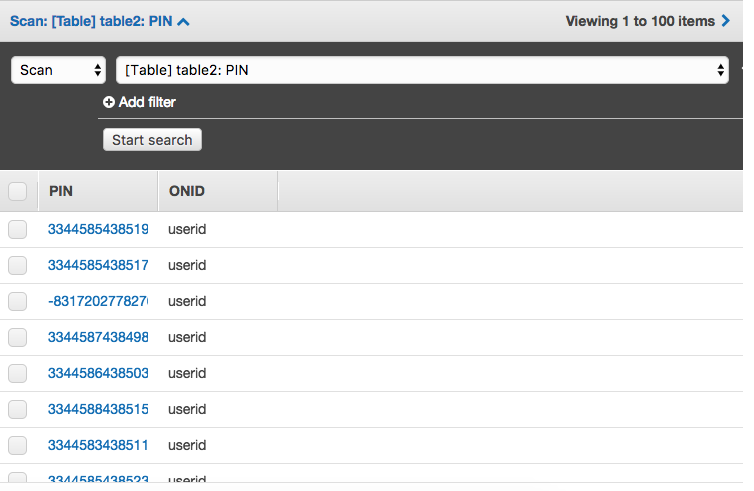
\includegraphics[width=15cm, height=8cm]{ONID.png}
\centering
\caption{result of ONID table}
\end{figure}
\begin{figure}[H]
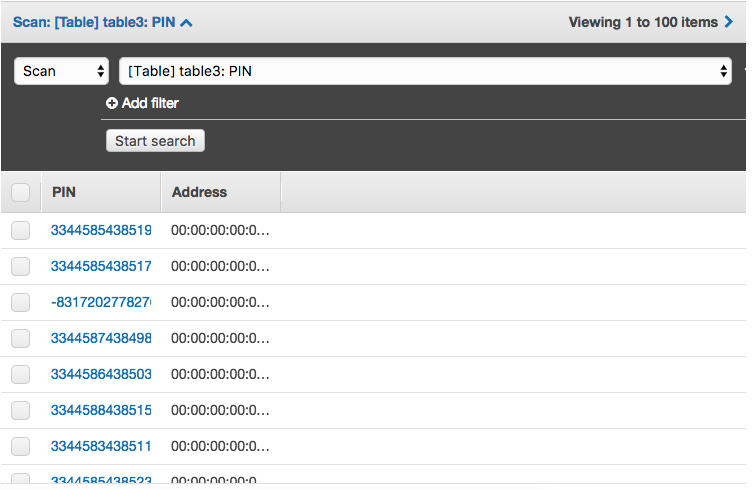
\includegraphics[width=15cm, height=8cm]{address.png}
\centering
\caption{result of Mac address table}
\end{figure}
\begin{figure}[H]
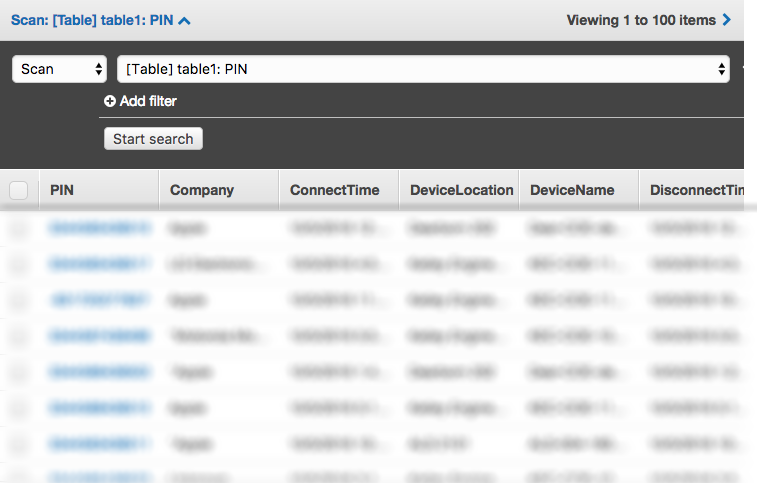
\includegraphics[width=15cm, height=8cm]{data.png}
\centering
\caption{result of Data table}
\end{figure}